\documentclass[10pt,twocolumn]{article}

\usepackage{times}
\usepackage{fullpage}

\usepackage{booktabs}  % for \midrule
%\usepackage{subfigure}
\usepackage{balance}
\usepackage{graphicx}
\usepackage{xspace}
%\usepackage{pslatex}
%\usepackage{pifont}
%\usepackage{multirow}
%\usepackage{array}
%\usepackage{booktabs}
%\usepackage{cite}
\usepackage{url}
%\usepackage{cancel}
\usepackage{color,colortbl}
%\usepackage{microtype}
%\usepackage{textcomp}% http://ctan.org/pkg/textcomp
\usepackage{tabularx}
\usepackage{framed}
\usepackage[]{algorithm2e}
\SetAlFnt{\small}
\SetAlCapFnt{\small}
\usepackage{algorithmic}

\usepackage{listings}
%\usepackage{scrextend}
%\usepackage{mathtools}
\usepackage{pbox}

\let\labelindent\relax
\usepackage{enumitem}

\usepackage{tikz}
\usetikzlibrary{arrows,automata}
\usetikzlibrary{calc,positioning}
\usepackage{lipsum,adjustbox}
\usepackage{float}

%\usepackage{tikz}
%\usepackage{decorations.pathmorphing}
%\usepackage{assymb}

\usepackage[labelfont=bf]{caption}

%\theoremstyle{plain}
\newtheorem{theorem}{\bf{Theorem}}%[section]
\newtheorem{lemma}[theorem]{\bf{Lemma}}
\newtheorem{corollary}[theorem]{\bf{Corollary}}
\newtheorem{proofl}[theorem]{\bf{Proof}}
\newtheorem{proposition}[theorem]{\bf{Proposition}}

%\theoremstyle{definition}
\newtheorem{definition}{\bf{Definition}}%[section]
\newtheorem{observation}{\bf{Observation}}%[section] 

%\theoremstyle{remark}
\newtheorem{example}{\bf{Example}}
\newtheorem{notation}{\bf{Notation}}
\newtheorem{fact}{\bf{Fact}}

\usepackage{listings}
%%\usepackage{listings-golang}
\usepackage{color}

%\usepackage{sectsty}
%\sectionfont{\fontsize{12}{15}\selectfont}


\newcommand\mypara[1]{\vspace{.3em}\noindent\textbf{#1}}
\newcommand{\urlwofont}[1]{\urlstyle{same}\url{#1}}


%%%%%%%%%%%%%%%%%%%%%%%%%%%%%%%%%%%%%%%%
% Useful reviewing/feedback annotations
\usepackage{ifthen}
\usepackage[normalem]{ulem} % for \sout
\usepackage{xcolor}
\usepackage{amssymb}

\newcommand{\ra}{$\rightarrow$}
\newboolean{showedits}
\setboolean{showedits}{true} % toggle to show or hide edits
\ifthenelse{\boolean{showedits}}
{
	\newcommand{\ugh}[1]{\textcolor{red}{\uwave{#1}}} % please rephrase
	\newcommand{\ins}[1]{\textcolor{blue}{\uline{#1}}} % please insert
	\newcommand{\del}[1]{\textcolor{red}{\sout{#1}}} % please delete
	\newcommand{\chg}[2]{\textcolor{red}{\sout{#1}}{\ra}\textcolor{blue}{\uline{#2}}} % please change
}{
	\newcommand{\ugh}[1]{#1} % please rephrase
	\newcommand{\ins}[1]{#1} % please insert
	\newcommand{\del}[1]{} % please delete
	\newcommand{\chg}[2]{#2}
}

\newboolean{showcomments}
\setboolean{showcomments}{true}
%\setboolean{showcomments}{false}
\newcommand{\id}[1]{$-$Id: scgPaper.tex 32478 2010-04-29 09:11:32Z oscar $-$}
\newcommand{\yellowbox}[1]{\fcolorbox{gray}{yellow}{\bfseries\sffamily\scriptsize#1}}
\newcommand{\triangles}[1]{{\sf\small$\blacktriangleright$\textit{#1}$\blacktriangleleft$}}
\ifthenelse{\boolean{showcomments}}
%{\newcommand{\nb}[2]{{\yellowbox{#1}\triangles{#2}}}
{\newcommand{\nbc}[3]{
 {\colorbox{#3}{\bfseries\sffamily\scriptsize\textcolor{white}{#1}}}
 {\textcolor{#3}{\sf\small$\blacktriangleright$\textit{#2}$\blacktriangleleft$}}}
 \newcommand{\version}{\emph{\scriptsize\id}}}
{\newcommand{\nbc}[3]{}
 \renewcommand{\ugh}[1]{#1} % please rephrase
 \renewcommand{\ins}[1]{#1} % please insert
 \renewcommand{\del}[1]{} % please delete
 \renewcommand{\chg}[2]{#2} % please change
 \newcommand{\version}{}}
\newcommand{\nb}[2]{\nbc{#1}{#2}{orange}}

\definecolor{ibcolor}{rgb}{0.4,0.6,0.2}
\newcommand\iv[1]{\nbc{IB}{#1}{ibcolor}}
\usepackage{wasysym}
\newcommand\yesml[1]{\nbc{ML {\textcolor{yellow}\sun}}{#1}{mircolor}}

%% here you can make your own annotations
\definecolor{sgcolor}{rgb}{0.2,0.0,0.5}
\newcommand\sg[1]{\nbc{SG}{#1}{sgcolor}}

\definecolor{hccolor}{rgb}{0.21,0.54,0.84}
\newcommand\hc[1]{\nbc{HC}{#1}{hccolor}}

\definecolor{ideacolor}{rgb}{1.0,0,0.5}
\newcommand\idea[1]{\nbc{IDEA}{#1}{ideacolor}}


\definecolor{abstractcolor}{rgb}{0.0,0.5,1.0}
\newcommand\rabstract[1]{\nbc{ABSTRACT}{#1}{abstractcolor}}

\definecolor{introcolor}{rgb}{0.0,1.0,0.5}
\newcommand\rintro[1]{\nbc{INTRO}{#1}{introcolor}}

\definecolor{papercolor}{rgb}{1.0,1.0,0.0}
\newcommand\rpaper[1]{\nbc{PAPER}{#1}{papercolor}}

\definecolor{multicolor}{rgb}{1.0,0,0}
\newcommand\rmulti[1]{\nbc{MULTI}{#1}{multicolor}}

% Todo Command
\definecolor{todocolor}{rgb}{0.9,0.1,0.1}
\newcommand{\todo}[1]{\nbc{TODO}{#1}{todocolor}}


%%%%%%%%%%%%%%%%%%%%%%%%%%%%%%%%%%%%%%%%


\begin{document}

%\title{Inferring likely data invariants of distributed systems}
\title{Title (found in paper.tex)}
\author{Authorname lastname and Author2 lastname2 \\ University of Califonia San Diego}
\date{}

\maketitle

\section{Pitch}

\todo{3-4 sentences descibing your plan at a high level}
\section{Proposal}

The body of your proposal. Below are some bullets for questions you should
answers within your proposal. Figure~\ref{fig:example} contains fake information
from a chart that will, with any luck contain some data from a measurement
you've taken. TaMake sure that you adhere to good academic standards and cite all
of the work relate to your project. For example if your project involves
performance isolation on SmartNICs you might want to cite~\cite{fairnic}. See
paper.bib for the format of \LaTeX references. Many academic papers will have
bibtex entries posted near where you can download their pdf's online.


\begin{itemize}
    \item{\todo{What is the question you want to answer}}
    \item{\todo{Why is it important}}
    \item{\todo{What is the related work}}
    \item{\todo{How do you plan to complete it?}}
    \item{\todo{What software artifact will you complete?}}
    \item{\todo{What software packages do you plan to use?}}
    \item{\todo{What is your evaluation plan?}}
\end{itemize}

\begin{figure}[H]
    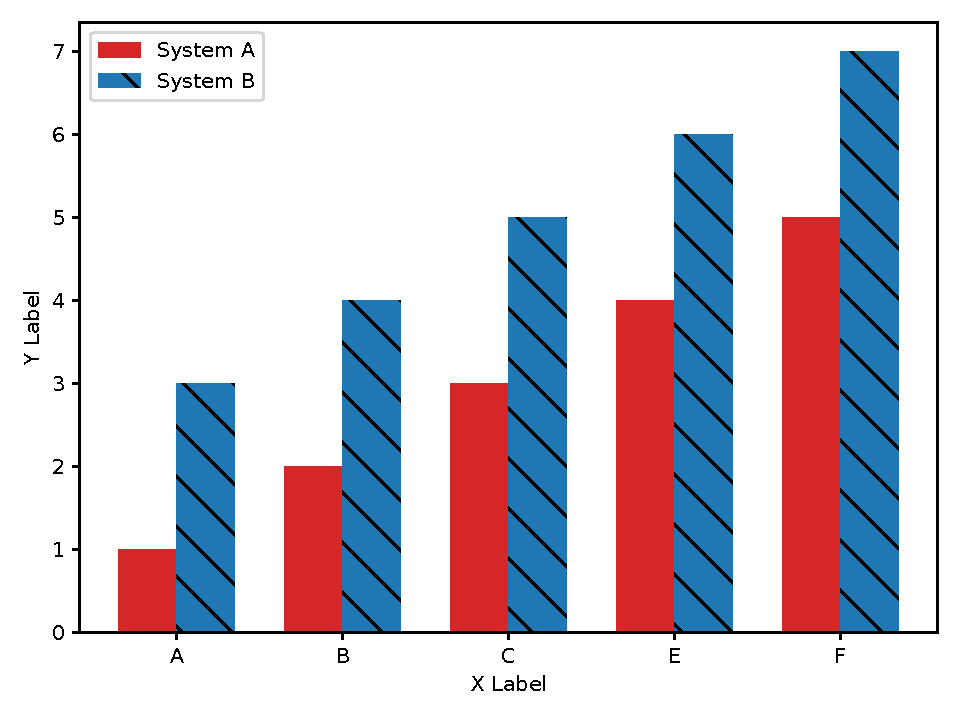
\includegraphics[width=0.45\textwidth]{fig/example.pdf}
    \caption{Example of a figure made with matplotlib. Found in fig/example.py. If you have a figure use vector graphics}
    \label{fig:example}
    %%remove a bit of whitespace under the figure (for space saving)
    \vspace*{-10.00mm}
\end{figure}

\begin{center}
    \begin{table}
    \begin{tabular}{ |c|c|c| }
    \hline
            & studied & $\neg$ studied \\ \hline
    Midterm & Pass 
\includegraphics{fig/check.png} & Skimmed by 
\includegraphics{fig/almost.png} \\ \hline
    Final   & Pass 
\includegraphics{fig/check.png} & See you next year 
\includegraphics {fig/fail.png} \\ \hline
    \end{tabular}
    \caption{Expected outcomes for various studying habits in 223B}
    \label{tab:studyhabits}
\end{table}
\end{center}


\section{timeline}

\begin{itemize}
    \item{Week 1}
    \item{Week 2}
    \item{Week 3}
    \item{Week 4}
    \item{Week 5}
    \item{Week 6}
    \item{(more or less weeks)}
\end{itemize}



\balance
\vspace{-0.3cm}
{\footnotesize \bibliographystyle{acm}
\bibliography{paper}}
\vspace{-0.5cm}

\end{document}
